\documentclass{article}
\usepackage{graphicx}
\usepackage{mathtools}
\usepackage{xfrac}
\usepackage{amsmath, amssymb}
\usepackage{listings}
\usepackage{float}
\usepackage{wrapfig}
\usepackage{tikz}
\usepackage{fullpage}
\usepackage{hyperref}
\usepackage{mathalpha}
\usepackage{tikz}
\usepackage{cite}
\usepackage{amsthm}

\newtheorem{theorem}{Proposition}[section]
\newtheorem{corollary}{Corollary}[theorem]
\newtheorem{lemma}[theorem]{Lemma}

\theoremstyle{definition}
\newtheorem{definition}{Definition}[section]

\theoremstyle{remark}
\newtheorem*{remark}{Remark}
\newtheorem*{example}{Example}
\newtheorem*{notation}{Notation}

\title{Statistical Physics I}
\author{Based on the lectures of Manuela Kulaxizi\\David Lawton}
\date{11th Sep. 2024.}

\begin{document}

\maketitle

\tableofcontents

\newpage

\section{Lecture: 1}

Thermodynamics can be defined as the study of the physical behaviours of macroscopic system properties. It is loosely defined in terms of a large number of constituents,$N$ ($\sqrt{N}>>1$). Behaviours arises as a consequence of physical laws, symmetries. Thermodynamics treats systems as approx. static. Macroscopic observations sense course spatial averages of the constiuents' motion.

\subsection[short]{Determining Appropriate Variables}
Focus on \textbf{simple, macroscopic} systems. Simple meaning homogeneous, isotropic and uncharged. The system must be large enough to not consider interactions at the boundaries of the system.
\begin{enumerate}
    \item $V$: \textbf{volume} of the system.
    \item $N_i$: \textbf{number of constituents} of system or subsystem $i$; chemical composition.
    \item $E$: \textbf{intrinsic energy} of the system.
\end{enumerate}
\vspace{0.5cm}
\hrule
\begin{theorem}[Postulate I]
    There exist states, \textbf{equilibrium states}, that are completely characterised by some variables of the system:
    \begin{equation}
        \lbrace V, N_i, E | i = 1,2,...,n\rbrace
    \end{equation}
    equilibrium states are defined in relation to the surroundings.
\end{theorem}
\hrule
\vspace{0.5cm}
\subsection[short]{Walls and Constraints (Boundaries)}
A thermodynamic description requires the specification of `walls', constraints that seperate the system from the surroundings, and provide boundary conditions.
\begin{figure}[H]
    \centering
    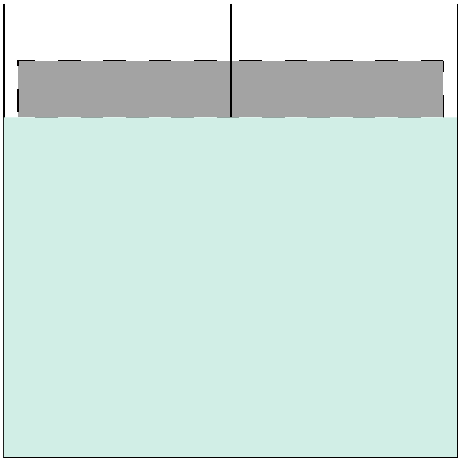
\includegraphics[width=0.5\textwidth]{/home/dj-lawton/Documents/Tikz/ThermoPump.png}
    \caption{\label{fig:ThermoPump}An example of a thermodynamic system, a gas under mechanical pressure.}
\end{figure}
In general, if a wall or boundary constrains an extensive variable, we call it \textbf{restrictive} w.r.t. that variable. Restriction of energy corresponds to thermal isolation ($E$ conserved), volume to mechanical isolation ($V=\text{const.}$), and number of constituents to chemical isolation ($N_i=\text{const.}$).
\vspace{0.5cm}
\hrule
\begin{theorem}[Postulate II]
    There exist walls, \textbf{adiabatic walls}, such that the work done in taking an adiabatically enclosed system between two equilibriuum states is determined entirely by the beginning and end states themselves, independent of external conditions, i.e. $W=\Delta E \equiv $ difference in intrinsic energy.
\end{theorem}
\hrule
\vspace{0.5cm}


\end{document}